Let us now discuss the effects of a join on homology. In the general case, there is not much we can conclude but it is still instructive. Assuming the same notation as before, note that $M$ can be broken down as a union of open subsets diffeomorphic to $M_1\setminus \iota_1(N)$ and $M_2\setminus \iota_2(N)$. We call these subsets $M_1^\circ$ and $M_2^\circ$ respectively. Then, their intersection can be viewed as a tubular neighborhood of $\S(\T M_i/\iota_i(N)) \to M$ (the $i$ does not matter here). 
\begin{definition}\label{def:framed-submanifold}
	Suppose $N\subset M$ is a submanifold and $F : N\times \R^{n-k} \to \T M /N$ a trivialization of its normal bundle. $F$ is said to be a \defn{framing}[framing of a manifold] of $N$ in $M$ and the pair $(N,F)$ said to be a \defn{framed submanifold} of $M$.
\end{definition}


Altering topology by surgery naturally ties into the next topic of cobordism in \cref{sec:cobordism}, a natural notion of equivalence for manifolds. While surgery might change the diffeomorphism type of a manifold, it does not change its cobordism type. This loose notion of equivalence allows us to fully classify manifolds up to cobordism -- something which is generally impossible for homeomorphism or diffeomorphism.\footnote{In high dimensions, classifying manifolds is an \defn{undecidable problem}, meaning there is no finite algorithm that will correctly match a manifold to a list of representatives.} We only briefly discuss surgery here, leaving elaboration to \cref{chap:h-cobordism} and \cref{chap:classification}.
% The determination of manifolds up to cobordism is also one of the entrypoints of homotopy theory into differential topology via the Thom-Pontryagin construction, a massively successful crossover which reduces hard geometric problems to (also admittedly hard) problems of computing homotopy groups. With each flavor of cobordism, a new homotopy problem emerges. Ultimately, it will turn out that most of the computational difficulty in computing the set of smooth structures on a sphere is as a result of these problems in homotopy theory.

\begin{remark}\label{rmk:characteristic-number-monomial-polynomial}
	Whenever we have some homogeneous decomposition $c=\sum_i c_i$ of a characteristic class and an $n$-dimensional manifold $M$, it is common to associate characteristic numbers of the tangent bundle to partitions $k_0|c_0|+k_1|c_1|+\cdots+k_\ell|c_\ell| = n$. Each such partition gives a degree $n$ homogeneous characteristic class $c_0^{k_0}\cdots c_\ell^{k_\ell}$. For each closed $n$-dimensional manifold $M$, the monomial $c_0^{k_0}\cdots c_\ell^{k_\ell}$ thus has an associated characteristic number $c_0^{k_0}\cdots c_\ell^{k_\ell}[M]$.

	More generally, given a polynomial in $\ell$ variables $K\in R[x_1,\ldots, x_\ell]$ with $K(z^{|c_0|}, \ldots, z^{|c_\ell|})$ homogeneous of degree $n$, the class $K(c_0,\ldots, c_\ell)$ is a homogeneous characteristic class of dimension $n$ and so has an associated characteristic number $K(c_0, \ldots, c_\ell)[M] \in R$.
\end{remark}

We can directly construct $M$ from $\pi_\R^1$ by taking the $M = S^1\times_{\Z/2} D^1$ to be the bundle associated to the action of $\Z/2$ by reflection on $D^1\subset \R$. There is also an embedding of $M$ into a surface we are familiar with -- in fact $M$ is homeomorphic to the complement of an open disk $\Int(D^2)$ in the real projective plane $\RP^2$.

Similarly to the real case, the total space of this associated bundle turns out to be a complex projective plane $\CP^2$ with an open disk $\Int(D^4)$ removed. Recall that $\CP^n$ can be formed inductively by glueing a $2n$-cell $D^{2n}$ to $\CP^{n-1}$ by the map $\pi_\C^{n-1} : \partial D^{2n} \to \CP^{n-1}$, this gives the usual cell structure on $\CP^n$ with a single cell in each even dimension.
We can arrange the open disk $\Int(D^4)$ being removed from $\CP^4 = S^2\cup_{\pi_\C^1} D^4$ to lie strictly in $D^4$. Removing this disk then gives a $D^2$-bundle over the boundary $S^2$.


The total space of this bundle is diffeomorphic to the complement of an open disk $\Int(D^8)$ in quaternionic projective plane $\HP^2$ by a similar argument to what was done in the complex case.

By letting $S^1\cong \U_1$ act as rotations on the complex unit disk $D^2\subset \C$, we get an associated $D^2$-bundle $E = S^3\times_{\U_1} D^2$.





Many of the matrices we're interested arise from trees in this way. For instance, the $E_8$ matrix defined in terms of the $E_8$ lattice in \cref{def:E8-lattice} arises from the Dynkin diagram for the exceptional Lie group $\E_8$.
\begin{proposition}
	The ${E_8}$ bilinear form is associated to the tree
	\[
		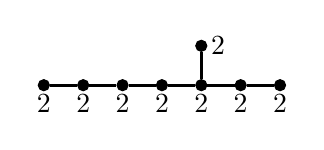
\begin{tikzpicture}
			\tikzset{dynode/.style={circle, draw, fill=black,
						minimum size=4pt, inner sep=0pt}}
			\tikzset{dyline/.style={line width=1pt}}
			\tikzset{dydash/.style={line width=1pt, dashed}}

			\begin{scope}[yshift=-10em, xshift=0]
				\node[dynode] (a1) at (0,0) {};
				\node[dynode] (a2) at (0.5,0) {};
				\node[dynode] (a3) at (1,0) {};
				\node[dynode] (a4) at (1.5,0) {};
				\node[dynode] (a5) at (2,0) {};
				\node[dynode] (a6) at (2.5,0) {};
				\node[dynode] (a7) at (3,0) {};
				\node[dynode] (a8) at (2,0.5) {};

				\draw[dyline] (a1) -- (a2) -- (a3) -- (a4) -- (a5) -- (a6) -- (a7);
				\draw[dyline] (a5) -- (a8);

				\node[below] () at (a1) {$2$};
				\node[below] () at (a2) {$2$};
				\node[below] () at (a3) {$2$};
				\node[below] () at (a4) {$2$};
				\node[below] () at (a5) {$2$};
				\node[below] () at (a6) {$2$};
				\node[below] () at (a7) {$2$};
				\node[right] () at (a8) {$2$};
			\end{scope}
		\end{tikzpicture}
		\quad\implies\quad
		\begin{pmatrix}
			2 & 1 &   &   &   &   &   &   \\
			1 & 2 & 1 &   &   &   &   &   \\
			  & 1 & 2 & 1 &   &   &   &   \\
			  &   & 1 & 2 & 1 &   &   &   \\
			  &   &   & 1 & 2 & 1 & 0 & 1 \\
			  &   &   &   & 1 & 2 & 1 & 0 \\
			  &   &   &   & 0 & 1 & 2 & 0 \\
			  &   &   &   & 1 & 0 & 0 & 2 \\
		\end{pmatrix}
	\]
	where each vertex of the tree is weighed by $2$.
\end{proposition}



\todo{give general conditions for representability}

\begin{theorem}[Preimage Theorem]\label{thm:preimage}
	If $f : N \to X$ is a smooth map transverse to a submanifold $M\subset X$ then $S=f^{-1}(M)\subset N$ is a submanifold with the same codimension in $N$ as $M$ in $X$.
\end{theorem}
\begin{proof}
	See the proof of Theorem~6.30 in \cite{lee2013smooth}.
\end{proof}

\begin{remark}\label{rmk:symmetric-preimage-theorem}
	We can get a symmetric version of this theorem as a straightforward corollary. If we have two transverse maps $f : N\to X$ and $g : M\to X$, then the map $f\times g : N\times M \to X\times X$ is transverse to the diagonal submanifold $\Delta\subset X\times X$. \cref{thm:preimage} will then imply that
	\[
		(f\times g)^{-1}(\Delta) \subset M\times N
	\]
	is a submanifold. When $g$ is an embedding, $(f\times g)^{-1}(\Delta)$ can be projected down onto $M$ to get the preimage $f^{-1}(M)$.
\end{remark}

If the manifolds involved in \cref{thm:preimage} are orientable, this preimage $S$ admits a canonical orientation by the following procedure. First of all, recall that for any embedded manifold $M\subset X$ there is an exact sequence of vector bundles by quotienting
\begin{equation}\label{eq:oriented-intersection-number-1}
	\begin{tikzcd}
		0 & {\TT M} & {\TT X}|_M & {\TT X/M} & 0
		\arrow[from=1-1, to=1-2]
		\arrow[from=1-2, to=1-3]
		\arrow[from=1-3, to=1-4]
		\arrow[from=1-4, to=1-5]
	\end{tikzcd}
\end{equation}
where $\TT X/M$ is the normal bundle of $M\subset X$. Using the orientations of $X$ and $M$, we can use this exact sequence to get an orientation of the normal bundle $\TT X/M$. At every point $p\in S$ of the preimage, the differential map $df$ connects the sequence \cref{eq:oriented-intersection-number-1} to the normal bundle sequence for the embedding $S\subset N$.
\begin{equation}\label{eq:oriented-intersection-number-2}
	\begin{tikzcd}
		0 & {\T_pS} & {\T_p N} & {\T_p N/S} & 0 \\
		0 & {\T_{f(p)}M} & {\T_{f(p)}X} & {\T_{f(p)}X/M} & 0
		\arrow[from=1-1, to=1-2]
		\arrow[from=1-2, to=1-3]
		\arrow["{df_p}", from=1-2, to=2-2]
		\arrow[from=1-3, to=1-4]
		\arrow["{df_p}", from=1-3, to=2-3]
		\arrow[from=1-4, to=1-5]
		\arrow["{df_p}", from=1-4, to=2-4]
		\arrow[from=2-1, to=2-2]
		\arrow[from=2-2, to=2-3]
		\arrow[from=2-3, to=2-4]
		\arrow[from=2-4, to=2-5]
	\end{tikzcd}
\end{equation}
In this diagram \cref{eq:oriented-intersection-number-2}, the rightmost vertical map is an isomorphism by the transversality of $f$ and $M$. This means that we can pullback the orientation on $\T_{f(p)} X/M$ to $\T_p N/S$. Since $\T_p N$ is oriented, the usual ``2-out-of-3'' rule applied to the top row of \cref{eq:oriented-intersection-number-2} gives an orientation of $\T_p S$. See \cref{fig:preimage-orientation} for an example of this orienting procedure.

\begin{figure}[ht]
	\centering
	\import{diagrams}{preimage-orientation.pdf_tex}
	\caption{Orienting a preimage (assuming a clockwise orientation on $X$ and $N$).}\label{fig:preimage-orientation}
\end{figure}

When $M$ and $N$ have complementary dimensions, the preimage $S=f^{-1}(N)\subset M$ is a compact oriented $0$-dimensional manifold. For each point $p\in S$, we have $\T_p S=0$ so the map $\T_p N\to \T_p N/S$ in \cref{eq:oriented-intersection-number-2} is an isomorphism. The orientation of $N$ gives an orientation of $\T_p N$, and the preimage orientation procedure gives us an orientation of $\T_p N/S$. Now we can define:

\begin{definition}
	The \defn{local intersection number}[oriented intersection number (local)] of $f$ and $M$ at $p\in S$ is
	\[
		I_p(f, M) = \begin{cases}
			+1 & \T_p N/S \textrm{ has the same orientation as } \T_p N,     \\
			-1 & \T_p N/S \textrm{ has the opposite orientation to } \T_p N.
		\end{cases}
	\]
\end{definition}
Summing over all of the local intersection numbers gives a global quantity.
\begin{definition}
	The \defn{(oriented) intersection number}[oriented intersection number] of a smooth map $f : N \to X$ intersecting a submanifold $M\subset X$ transversally is
	\[
		I(f, M) = \sum_{p\in S} I_p(f, M) \in \Z.
	\]
\end{definition}

\begin{remark}\label{rmk:symmetric-intersection-number}
	For a more symmetric version of this definition when two smooth maps $f : N \to X$ and $g : M \to X$ intersect transversally, we use \cref{rmk:symmetric-preimage-theorem} to define the oriented intersection number of the smooth maps $f$ and $g$ as
	\[
		I(f,g) = I(f\times g, \Delta).
	\]
	This symmetric intersection number is graded-commutative in the dimensions of $M$ and $N$:
	\begin{equation}\label{eq:intersection-number-graded-commutative}
		\#^X(f,g) = (-1)^{\dim M\cdot \dim N} \#^X(g,f)
	\end{equation}
\end{remark}

Just as the property of transversality is stable -- resilient to homotopic perturbations -- so too is the oriented intersection number. This follows as a corollary to a more general theorem.

\begin{theorem}
	If $W$ is a compact oriented manifold with boundary, and $H : W \to X$ is a smooth map, then $\#^X(\partial H, M)=0$. Here, we use the notation $\partial H : \partial W \to X$ to refer to the restriction of $H$ to the boundary of $W$.
\end{theorem}

\begin{corollary}
	If $H : [0,1]\times N \to X$ is a smooth homotopy, then $I(H_0, M) = I(H_1, M)$.
\end{corollary}

\begin{remark}
	If we don't assume orientations, we can still get a homotopy invariant intersection number, however we must reduce mod $2$. In this case, we could simply define
	\[
		\widetilde{I}(f,M) = |S|\mod 2.
	\]
	This is called the \defn{unoriented intersection number}.
	\todo{elaborate}
\end{remark}



\begin{theorem}[Morse Inequality]
	Let $M^n$ be a closed manifold with $f : M\to \R$ a Morse function. Let $\beta_i=\rank \H_i(M)$ be the $i$-th Betti number of $M$ and let $c_i$ be the number of critical points of $f$ of index $i$. Then, for every $\ell\in \Z^{\geq 0}$ we have
	\begin{equation}
		\beta_\ell - \beta_{\ell-1} + \beta_{\ell-2} - \cdots +(-1)^\ell \beta_0 \leq c_\ell - c_{\ell-1} + c_{\ell-2} - \cdots + (-1)^\ell c_0.
	\end{equation}
\end{theorem}


\begin{proposition}\label{prop:leading_coefficient_L_genus}
	The leading coefficient of the $L$-genus $L_k$ is $s_k=2^{2k}(2^{2k-1}-1)B_{2k}/(2k)!$
\end{proposition}
\begin{proof}
	From a formula of Cauchy, we can derive a generating function for $s_k$ by
	\[
		1-t\frac{d\log Q_L(\sqrt{t})}{dt} = 1-\frac{1}{3}t + \frac{7}{45}t^2-\frac{62}{945}t^3+\frac{127}{4725}t^4-\cdots = \sum_{k\geq 0} (-1)^{k}s_k t^k.
	\]
	For more details, see Problem 19-B and 19-C of \cite{milnorstasheff1974}.
\end{proof}
